\documentclass[11pt,a4paper]{article}
\usepackage[T1]{fontenc}
\usepackage{lmodern}
\usepackage[margin=27mm,headheight=15pt]{geometry}
\usepackage{amsmath,amssymb,amsthm,mathtools}
\usepackage{booktabs,longtable,array,tabularx}
\usepackage{graphicx,xcolor,microtype}
\usepackage{enumitem,listings,fancyhdr}
\usepackage[hyphens]{url}
\usepackage[colorlinks=true,linkcolor=blue!45!black,citecolor=blue!45!black,urlcolor=blue!45!black]{hyperref}
\usepackage{cleveref}
\definecolor{ink}{RGB}{24,43,65}
\definecolor{muted}{RGB}{72,88,102}
\definecolor{light}{RGB}{242,246,249}
\pagestyle{fancy}
\fancyhf{}
\fancyhead[L]{\small\textcolor{muted}{Support-sensitive unknot certificates}}
\fancyhead[R]{\small\textcolor{muted}{ProveIt research continuation}}
\fancyfoot[C]{\thepage}
\renewcommand{\headrulewidth}{0.3pt}
\newtheorem{theorem}{Theorem}[section]
\newtheorem{lemma}[theorem]{Lemma}
\newtheorem{proposition}[theorem]{Proposition}
\newtheorem{corollary}[theorem]{Corollary}
\theoremstyle{definition}
\newtheorem{definition}[theorem]{Definition}
\newtheorem{remark}[theorem]{Remark}
\newcommand{\Q}{\mathbb Q}
\newcommand{\Z}{\mathbb Z}
\newcommand{\R}{\mathbb R}
\newcommand{\F}{\mathbb F}
\newcommand{\supp}{\operatorname{supp}}
\newcommand{\rank}{\operatorname{rank}}
\newcommand{\bits}{\operatorname{bits}}
\newcommand{\nnz}{\operatorname{nnz}}
\newcommand{\calK}{\mathcal K}
\newcommand{\calT}{\mathcal T}
\newcommand{\code}[1]{{\small\nolinkurl{#1}}}
\lstset{basicstyle=\ttfamily\small,backgroundcolor=\color{light},frame=single,
 rulecolor=\color{light},breaklines=true,columns=fullflexible,keepspaces=true,
 showstringspaces=false,xleftmargin=5pt,xrightmargin=5pt,aboveskip=10pt,belowskip=10pt}
\setlist{itemsep=3pt,topsep=5pt}
\setlength{\emergencystretch}{2em}
\hypersetup{pdftitle={Support-Sensitive Certificates for Unknot Recognition},
 pdfauthor={ProveIt research continuation, prepared with ChatGPT},
 pdfsubject={Exact coordinate transport, support nullity, ray peeling, and a quasi-polynomial research agenda}}

\title{\textcolor{ink}{Support-Sensitive Certificates\\for Unknot Recognition}\\[6pt]
 \large Optimal coordinate transport, component profiles,\\and linear unit-pivot ray certificates}
\author{Research continuation prepared for Vladimir Reshetnikov\\
 \small ProveIt project; mathematical development and implementation with ChatGPT}
\date{9 October 2026}

\begin{document}
\maketitle
\begin{abstract}
We develop exact, independently checkable improvements to the normal-surface
analysis stage of ProveIt's unknot recognizer.  For a supplied admissible normal
vector $x$, let $d$ be the nullity of the matching equations after all zero
coordinates of $x$ have been fixed.  We compile a decoder from exactly $d$
selected coordinates, minimize its allocated binary-slot cost by a weighted
matroid basis calculation, and transport the selected data as one scalar.
A fibre invariant proves that scalar packing preserves every canonical weight
run of the corresponding vector calculation.  We sharpen the bound on distinct
full component-coordinate types to $H(x)\le 2d-a$, where $a$ counts supported
vertex links, and to $H(x)\le d$ when all components are two-sided.

A second path partitions the source by actual face-arc incidences and counts
essential discs on rank-one blocks without an interval-orbit computation.
An integral unit-pivot peeling certificate proves rank one and recovers the
primitive generator from a single coordinate.  For the entire layered
Fibonacci meridian family it has exactly $3t-1$ steps in $t$ tetrahedra,
despite exponentially many represented normal pieces.  The deliverable
contains additive Python implementations, independently written checkers,
adversarial tests, a reproducible corpus audit, paired benchmarks, and a
diagram-bound positive-certificate interface.

These are local supplied-surface results.  Compressed component extraction and
primitive vertex-surface connectedness are classical antecedents, explicitly
credited here.  We do not prove a quasi-polynomial bound for unrestricted unknot
recognition.  We identify the remaining selection, hierarchy, marking, and
representation bounds needed for such a theorem and formulate concrete next
research targets.
\end{abstract}

\vspace{4pt}
\noindent\textbf{Reproducibility baseline.}
\href{https://github.com/VladimirReshetnikov/ProveIt/tree/3a90fb34146c915328ab8eac6250cc2514f74ed0/Topology/UnknotRecognition}{ProveIt},
commit \code{3a90fb34146c915328ab8eac6250cc2514f74ed0}.
All performance statements refer to the accompanying executable experiment,
not to an unspecified later revision.

\clearpage
\begingroup
\small
\tableofcontents
\endgroup
\newpage

\section{The problem addressed and the contribution boundary}
\label{sec:scope}

The long-term goal is a deterministic unknot recognizer whose running time,
on a diagram with $n$ crossings, is $2^{(\log n)^{O(1)}}$.  A useful continuation
must improve a concrete part of the algorithm while keeping the distinction
between a local polynomial routine and the global search explicit.  A normal
surface can contain exponentially many elementary discs and yet have a short
binary coordinate vector.  Operating on those coordinates is indispensable,
but does not by itself determine which surface recognition should examine.

This article concentrates on two questions that the maintained implementation
already exposes as precise computational interfaces:
\begin{enumerate}
\item Given a normal vector, what are the distinct complete coordinate vectors
of its connected components, with binary multiplicities?
\item How many of its components are discs with essential boundary on the
boundary torus?
\end{enumerate}
The first question needs more information than the second.  Our implementation
uses a compiled coordinate observer for the first, and a rank-one algebraic
shortcut with an exact fallback for the second.  An additional wrapper binds
a positive answer to the canonical exterior of a particular classical knot
diagram.  It accepts supplied normal coordinates; it does not search for them.

\subsection{What the pinned repository and incoming work already contain}

The audit covered the maintained Python implementation and synthesis sources,
and the relevant incoming archives at the pinned commit.  The maintained
coordinate census already transports positive quadrilateral coordinates and
one positive minimum triangle anchor per supported vertex link.  Its dimension
is essentially $q+a$, where $q$ counts positive quadrilateral types.  Its
decoder is sparse and integral.  Replacing it with generic linear algebra is
therefore a tradeoff, not an automatic improvement.

The maintained code also contains exact three-weight essential-disc detection,
an independent orbit replay checker, primitive-core disc counting, a canonical
diagram-to-exterior construction and independent local verification, and
minimum-span cocycle optimization with a forced-difference quotient.  Earlier
synthesis establishes component-type bounds using quadrilateral coordinates.
The incoming support-kernel package already develops small supported systems,
primitive-ray certificates, low-nullity ray enumeration, and dense Fibonacci
examples.  We do not claim these as new discoveries.  The accompanying
provenance manifest names the inspected files and incoming archive hashes.

The additions here are a cost-optimal observer on the \emph{actual positive
standard-coordinate support}, a scalar realization with an exact live-state
invariant, the $2d-a$ inventory refinement, safe geometric support blocks, and
an executable unit-pivot specialization that proves and exploits the integral
ray structure without Gaussian elimination.  Their composition with existing
source correspondence is also implemented and tested.

\subsection{Classical and current external context}

Agol--Hass--Thurston already give compressed component coordinates for a
supplied normal surface in time polynomial in triangulation size and logarithmic
normal weight \cite[Theorem~16, Corollary~17]{AHT06}.  Our observer and packing
refine that local calculation.  Hass--Lagarias--Pippenger use active-constraint
rank and primitivity to certify vertex-surface connectedness without tracing
all pieces \cite[Lemma~5.3, Sections~6 and~8]{HLP99}.  Our ray path specializes
that established principle.  Weighted-basis optimization is the matroid greedy
theorem \cite{Edmonds71}; the contribution is the exact objective and certified
application to this implementation.

Lackenby's inspected 2021 Oxford handout announces
$2^{O((\log n)^3)}=n^{O((\log n)^2)}$ \cite[pp.~7, 25]{Lackenby21Slides}.
The July 2026 preprint gives new hierarchy and certification results.
Its step-visit bound is $L(g+1)^L$, but individual step costs are not all
specified; it does not assert a quasi-polynomial total bound
\cite[Sections~9--10]{Lackenby26}.  We use this distinction to formulate a
precise global accounting target in \cref{sec:global}, rather than infer a
complexity theorem from a local benchmark.

\section{Input model, support, and what a certificate means}
\label{sec:model}

Let $\calT$ be a finite triangulation with $t$ tetrahedra, given by face
pairings.  For disc queries we require the maintained validator's contract:
a connected compact orientable $3$-manifold, one torus boundary component,
and spherical or disc vertex links.  The linear and component-profile
arguments need the usual normal-coordinate uniqueness and connected vertex
links; they do not need a knot-diagram origin.  The source-bound interface
adds that origin separately.

Let $x\in\Z_{\ge0}^{7t}$ satisfy the matching equations and quadrilateral
constraints.  Write $F(x)$ for its normal realization, unique up to normal
isotopy \cite[Theorem~5.1]{HLP99}.  Each connected component has a nonzero vector $y$ with
$0\le y\le x$.  Set
\begin{equation}
 S=\{i:x_i>0\},\quad s=|S|,\quad
 A=A_S,\quad r=\rank_{\Q} A,\quad d=s-r,\quad
 \calK_S=\ker_{\Q} A.                         \label{eq:support}
\end{equation}
Here $A_S$ restricts the full matching matrix to the columns in $S$.
There are at most $6t$ rows and at most $5t$ supported columns.  Every original
row has the form $T+Q-T'-Q'=0$.  After coincident terms cancel, its nonzero
coefficients are $\pm1$ and its Euclidean norm is at most $2$.

Since $x$ is positive on $S$, the nonnegative cone in $\calK_S\otimes\R$
has relative dimension $d$.  Indeed a small neighbourhood of $x$ within this
space stays positive.  Thus $d$ is the actual dimension of the supported
solution face, not merely a dimension of a larger quadrilateral sector.
For $x=0$ we use $S=\varnothing$ and $s=r=d=0$.

Let $B=\max_{i\in S}\bits(x_i)$, with $B=0$ for the empty source, and let
$W=\sum_i x_i$.  Binary input length is bounded above by
$O(t\log(t+1)+sB)$ bits, with actual coordinate length
$\sum_{i\in S}\bits(x_i)$;
$\log(W+1)=O(B+\log(t+1))$.  Unit-cost arithmetic on a $B$-bit integer is
not a bit-complexity model.  We state structural operation counts separately
from costs of reading, adding, multiplying, or decoding these integers.

\begin{definition}[Component profile]
The full component profile is the finite map sending each distinct complete
$7t$-coordinate vector $y$ of a connected component to its multiplicity in
$F(x)$.  Its support size is $H(x)$.  Equal homeomorphism types with different
normal coordinates are distinct entries.
\end{definition}

A certificate in this work is an exact finite object checked against the
original triangulation and source coordinates.  Producers can be complicated
or heuristic.  Acceptance depends on a separately implemented replay of
algebraic identities and the maintained finite geometry and orbit contracts.
This is an independently checked implementation, not a proof-assistant
formalization or a claim that the entire Python runtime is formally verified.

\section{An optimal coordinate observer on the source support}
\label{sec:observer}

\subsection{Dimension and minimum binary-slot cost}

For $i\in S$ put $b_i=\bits(x_i)=\lceil\log_2(x_i+1)\rceil$.
A retained coordinate needs a slot of this width to hold every value in
$[0,x_i]\cap\Z$.  For $J\subseteq S$, let $\pi_J$ be coordinate restriction.

\begin{theorem}[Minimum-cost support projection]
\label{thm:optimal}
The map $\pi_J$ is injective on $\calK_S$ if and only if the columns of $A$
indexed by $S\setminus J$ are independent.  In particular, an injective
coordinate projection of minimum total cost $\sum_{j\in J}b_j$ retains exactly
$d$ coordinates.  A minimum is obtained by greedily taking independent pivot
columns in nonincreasing order of $b_i$ and retaining their complement.
\end{theorem}

\begin{proof}
A nonzero vector in $\ker A$ with zero restriction to $J$ is exactly a nonzero
linear dependence among the complementary columns.  This proves the first
claim.  All costs are positive, so a cost-minimizing complement extends to a
column basis; otherwise removing another retained coordinate decreases cost.
Its size is $r$, and the retained size is $d$.

Minimizing the retained sum is equivalent to maximizing the pivot sum, because
their sum is the fixed total $\sum_{i\in S}b_i$.  Column independence forms a
representable matroid.  For completeness, take a maximum-weight basis
containing the current greedy prefix.  If the next accepted greedy column is
absent, the fundamental circuit obtained by adding it contains a basis column
outside the prefix that may be exchanged out.  Such a column has no greater
weight: an earlier rejected column was already spanned by an earlier prefix.
The exchange preserves maximum weight and extends the greedy prefix.  Induct
until the greedy basis is installed.  Its complement gives the desired
minimum.  Ties are broken by coordinate index for reproducibility.
\end{proof}

\begin{corollary}[Comparison with the maintained observer]
\label{cor:oldobserver}
Let $q$ count positive quadrilateral types and let $a$ count supported vertex
links.  Then $d\le q+a$, and the new minimum slot budget is no greater than
that of the maintained positive-quadrilateral/vertex-anchor observer.
\end{corollary}
\begin{proof}
Retain all positive quadrilaterals and one triangle coordinate for each fully
supported vertex link.  A kernel vector vanishing on these coordinates has
zero quadrilaterals.  Triangle matching then makes its triangle heights
constant around each connected vertex link.  That constant is zero either
because an unsupported triangle was fixed to zero or because its retained
anchor is zero.  Thus the retained projection is injective.  Apply
\cref{thm:optimal} to this feasible coordinate set.
\end{proof}

The optimality domain matters.  This minimizes allocated binary slots among
coordinate projections admitting a linear decoder on the whole supported
matching space.  It does not optimize arbitrary finite encodings, decoder
sparsity, or total runtime.  A single huge integer can encode a finite box.
Nor is $d$ necessarily the dimension of the finite set of components appearing
in this one source.  For genuine mixed-radix bases $x_j+1$, minimizing their
product instead uses greedy weights $\log(x_i+1)$, equivalently the order of
$x_i$.  The shipped implementation optimizes binary slots.

\subsection{Exact decoder and independent rank evidence}

Let $P=S\setminus J$ be the pivot basis.  Choose $r$ original rows $R$ for which
$M=A[R,P]$ is nonsingular, put $C=A[R,J]$, and let $\Delta=\det M\ne0$.
The rational decoder is
\begin{equation}
 T[J,:]=I_d,\qquad T[P,:]=-M^{-1}C,\qquad
 D=|\Delta|,\qquad N=DT.                       \label{eq:decoder}
\end{equation}
It sends retained values $w$ to $Nw/D$.  We need not ask a checker to trust
the elimination that produced $N$.

\begin{theorem}[Certified support decoder]
\label{thm:decoder}
Suppose a certificate supplies complementary sets $J,P$, rows $R$, an integer
$D>0$, an integer matrix $N$, and evidence that $A[R,P]$ is nonsingular.  If
\[
 |J|=d,\quad |P|=|R|=s-d,\quad
 N[J,:]=D I_d,\quad AN=0,
\]
then $\dim\ker A=d$ and every $y\in\ker A$ equals $N y_J/D$.
For standard normal matching matrices a certificate of this form exists with
\[
 1\le D\le2^r,\qquad |N_{ij}|\le2^r.
\]
\end{theorem}

\begin{proof}
The identity rows make the $d$ columns of $N$ independent; $AN=0$ puts them in
the kernel.  Hence nullity is at least $d$.  The nonsingular $(s-d)$-minor gives
rank at least $s-d$, so equality holds in both bounds.  If $y$ is in the
kernel, $y-Ny_J/D$ is also in the kernel and vanishes on $J$.  The pivot minor
forces its remaining coordinates to vanish.

For existence use \cref{eq:decoder}.  Cramer's rule expresses each entry of
$N$ as a signed $r$-minor, with at most one pivot column replaced by a retained
column.  Every row of each such minor has norm at most $2$.  Hadamard's
inequality bounds its determinant by $2^r$.  The identity rows obey the same
bound.  When $r=0$, take $D=1$, $N=I_s$, and the empty minor.
\end{proof}

The rank evidence consists of a modulus $m\ge2$ and the claimed minor.  The
checker performs its own modular elimination and only inverts pivots whose
greatest common divisor with $m$ is $1$.  Successful elimination makes the
determinant a unit modulo $m$, and thus a nonzero integer.  Primality is not a
soundness assumption.  In particular, merely testing that a pivot is nonzero
modulo a composite modulus would be insufficient.

The producer chooses a small prime not dividing $D$.  Here is a self-contained
polynomial value bound.  For $r\ge1$ put $M_0=16(r+1)^2$.  If every prime at
most $M_0$ divided $D\le2^r$, there would be at most $r$ such primes, and
$\operatorname{lcm}(1,\ldots,M_0)\le M_0^r$.  The central binomial coefficient
$\binom{M_0}{M_0/2}$ divides this least common multiple: for each prime its
valuation is a sum of terms
$\lfloor M_0/p^k\rfloor-2\lfloor(M_0/2)/p^k\rfloor\in\{0,1\}$.
But that coefficient is at least $2^{M_0}/(M_0+1)\ge2^{M_0/2}$, whereas
$M_0/2>r\log_2 M_0$.  This is a contradiction.  Some prime at most $M_0$
therefore avoids $D$, and trial generation and divisibility testing are
polynomial.  For $r=0$, $D=1$ and modulus two suffices.  A bound merely on
the bit length of the final modulus would not establish this search bound.

The certificate stores $O(sd(r+1)+t\log(t+1))$ bits, including the dense
decoder and indices.  Sparse fraction-free elimination is performed separately
on algebraic column blocks.  With $m_A\le6t$ original matching rows, a
conservative dense estimate is $O(m_A s r)$ arithmetic operations on
polynomial-size minors.  Schoolbook
integer arithmetic gives a polynomial bound, for example $O(t^5)$ for the
elimination part; source input and output decoding are additional.  This
coarse upper bound is deliberately not a prediction of measured time.

For a recovered component, the checker computes $Nw$, checks every exact
division by $D$, and verifies $0\le y_i\le x_i$.  The numerators have
$O(B+r+\log(d+1))$ bits.  Arbitrary integer weights need not decode integrally:
the divisibility test is essential.  Reusing a valid decoder on another source
with the same positive support preserves correctness, but its original
minimum-cost claim need not survive changed coordinate magnitudes.

\begin{corollary}[Near-optimal reuse under uniform scaling]
\label{cor:scaling}
If a $d$-coordinate projection is minimum-slot for $x$, its slot cost for
$mx$, with integer $m\ge1$, exceeds the new optimum by at most $d$ bits.
\end{corollary}
\begin{proof}
For every positive coordinate,
$\bits(mx_i)=\bits(x_i)+\bits(m)-1+\varepsilon_i$ with
$\varepsilon_i\in\{0,1\}$.  Compare the old optimal set $J$ with a new optimal
set $J'$.  Both have $d$ coordinates, so the common term
$d(\bits(m)-1)$ cancels.  Old optimality gives
$\sum_J\bits(x_i)-\sum_{J'}\bits(x_i)\le0$, and the difference of the two
epsilon sums is at most $d$.  The claimed bound follows.
\end{proof}

\section{One scalar weight, with an invariant throughout transport}
\label{sec:packing}

Order $J=(j_1,\ldots,j_d)$ and set
\begin{equation}
 \sigma_1=0,\quad \sigma_k=\sum_{\ell<k}b_{j_\ell},\quad
 L=\sum_{k=1}^d b_{j_k},\quad
 E(y)=\sum_{k=1}^d y_{j_k}2^{\sigma_k}.       \label{eq:packing}
\end{equation}
For every integer $0\le y\le x$, the digits of $E(y)$ recover $y_J$ without
carries.  Furthermore $K=E(x)<2^L$.  Assign weight $2^{\sigma_k}$ to one
designated corner of each normal disc of type $j_k$, and zero otherwise.
The weight of a component is exactly $E(y)$.

This construction is an additive linear weight before it is a digit encoding.
That distinction permits use of the maintained weighted interval algorithm.
It also lets us prove more than final-output correctness.

\begin{theorem}[Packing preserves live weight runs]
\label{thm:packing}
Run vector-valued and packed scalar-valued weighted transport with the same
retained coordinates and the same interval-orbit trace.  At every stage each
live representative carries the sum of original weights over a fibre of
original points.  Distinct live fibres and emitted completed orbits are
disjoint.  Every live retained vector is consequently in $[0,x_J]$, its scalar
is in $[0,K]$, and the two representations have exactly the same canonical
constant-weight run partition.
\end{theorem}

\begin{proof}
Initially each fibre is a singleton.  Changes to the pairing description
preserve fibres.  When a truncation or fold removes points, the weight of a
removed fibre is transferred to its retained image.  The operation unions
disjoint fibres; translation and reflection formulas calculate these unions
without enumerating the points.  Completed static orbits are emitted and
removed.  Induction gives a partition of the original contributions into
live and emitted fibres.

There are exactly $x_{j_k}$ original unit contributions of coordinate $j_k$.
No fibre can contain more than all of them.  Hence each live vector lies in
the box where binary packing is injective.  Additivity gives the scalar as
$E$ of that vector and conserves total mass $K$.  Two adjacent live vectors
are equal if and only if their scalar encodings are equal.  Canonical merging
therefore creates precisely the same run boundaries in both representations.
\end{proof}

The code's signed difference arrays are an implementation device; they are
not live component vectors.  A conservative bound on their temporary values
is a polynomial in the number of runs and endpoint counts times $K$.  With
$R$ runs and initial interval size $N_0$, their bit length is
$O(L+\log(R+1)+\log(N_0+1))$.  Compressed weighted-orbit analysis remains
polynomial in the encoded input parameters \cite{AHT06}.

This theorem isolates two effects.  Switching from the old $q+a$ observer to
the support observer can change run counts.  Switching from the new $d$-vector
observer to its packed scalar cannot change them.  Any runtime difference in
the second comparison comes from arithmetic representation and allocation,
not a different combinatorial orbit problem.

Packing does not prove a factor-$d$ bit-operation improvement: an addition
on an $L$-bit integer can cost as much as the relevant collection of shorter
additions.  It can nevertheless reduce Python tuple creation, per-coordinate
loops, and hashing overhead.  Basis construction, exact decoding, and proof
replay must be included when assessing a complete query.  The old sparse
decoder can be preferable when $d$ is not much smaller than $q+a$.

\section{A sharper bound on the number of component types}
\label{sec:profiles}

For a quotient vertex $v$, let $\ell_v$ be its connected vertex-link vector.
Let $a$ count the vertices for which $\supp(\ell_v)\subseteq S$.  These are
exactly the vertex-link types occurring in $F(x)$: their common minimum
triangle height can be realized by small disjoint links, while a missing
required triangle forbids the type.  They are two-sided.  Every connected
triangle-only normal surface is a vertex link under the vertex-link hypotheses.

\begin{lemma}[Independence of disjoint two-sided types]
\label{lem:independence}
Distinct full normal-coordinate vectors of mutually disjoint connected
two-sided normal surfaces are linearly independent over $\Q$.
\end{lemma}

\begin{proof}
An alleged rational dependence can be cleared to an integer one.  Nonzero
normal vectors have nonnegative entries, so a nontrivial dependence has
coefficients of both signs.  Rearranging gives equality of two positive
integer combinations of distinct vectors.  Because the surfaces are
two-sided and mutually disjoint, each combination is realized by a disjoint
union of the indicated numbers of parallel copies.  Equal admissible normal
vectors determine normally isotopic surfaces, and that isotopy gives equal
multisets of connected full-coordinate types.  The two disjoint collections
of types in the dependence cannot have equal multisets.  This is a contradiction.
\end{proof}

\begin{theorem}[Support-nullity profile bound]
\label{thm:profile}
For every supplied normal vector in the stated manifold setting,
\begin{equation}
 H(x)\le 2d-a.                                \label{eq:profile}
\end{equation}
If all its components are two-sided, then $H(x)\le d$.
\end{theorem}

\begin{proof}
The two-sided assertion follows immediately from \cref{lem:independence},
since every component vector belongs to the $d$-dimensional supported space.

For the general assertion retain the $a$ link types separately.  For each
nonlink type choose one actual component of $F(x)$.  A two-sided representative
stays as it is.  Replace a one-sided representative by the boundary of a small
normal interval neighbourhood, with vertical boundary in the ambient boundary.
Its connected two-sided horizontal frontier has vector twice the original
vector.  Neighbourhoods can be chosen disjoint from all
other selected representatives and from the vertex links.  Coalesce equal
resulting vectors, and let $h$ be their number.

Each resulting nonlink vector $z$ has at most two original preimages: the
two-sided type $z$ and the one-sided type $z/2$.  It cannot become a link type,
because its positive quadrilateral coordinates survive doubling.  Thus
$H(x)-a\le2h$.  The $h$ distinct resulting types together with the $a$ links
are independent by \cref{lem:independence}, so $h+a\le d$.  Combining gives
$H(x)\le a+2(d-a)=2d-a$.  The empty source satisfies the statement by convention.
\end{proof}

This refines the proof mechanism already used in the repository's
\code{synthesis/compact_coordinates.tex}; it replaces a quadrilateral-count
dimension estimate by the exact supported nullity.  The factor two is needed.
In the one-tetrahedron solid-torus fixture, the primitive one-sided M\"obius
band has vector $M=(0,0,0,0;0,1,0)$.  Its source $3M$ has the central M\"obius
band and its connected double as two coordinate types, with $d=1$ and $a=0$.
Adding the disjoint vertex link $\ell=(1,1,1,1;0,0,0)$ gives
$(d,a,H)=(2,1,3)$.  These specific configurations are checked in the supplied
finite fixtures; primitivity of an arbitrary M\"obius band does not imply
support nullity one.

The bound concerns unmarked coordinate inventories.  It does not bound the
number of ways marked boundary arcs, parallelity data, or future hierarchy
attachments can distinguish otherwise identical components.  Using it as
a bound on global branch count requires a further theorem about those markings.

\section{Geometric blocks and exact essential-disc counts}
\label{sec:rays}

\subsection{A conservative partition from original face incidences}

Build a graph whose vertices are positive normal-disc types.  For every
original face-arc equation, connect all its positive participating types
before like terms are collected or cancelled.  Let $S_1,\ldots,S_b$ be the
connected blocks, and let $x^{(j)}$ be $x$ restricted to $S_j$ and zero elsewhere.

\begin{theorem}[Geometric support blocks]
\label{thm:blocks}
Each $x^{(j)}$ is an admissible matching vector, and
\[
 F(x)=\bigsqcup_{j=1}^{b}F(x^{(j)})
\]
up to normal isotopy.  The corresponding supported matching spaces form a
direct sum, so $d=\sum_j d_j$.
\end{theorem}

\begin{proof}
All positive occurrences of a single original matching equation belong to
one graph block.  Restricting to any block therefore either keeps that whole
equation on the source or sets both sides to zero.  Matching and quadrilateral
constraints follow.

An actual connection of normal discs across a face pairs arcs appearing in
one original face equation.  Their types lie in the same block.  Following
a connected component never leaves its block.  Within a tetrahedron the
normal discs themselves are disjoint, and the block restriction keeps exactly
the selected subcollection.  This proves the asserted disjoint union.  Finally,
no collected matching equation has supported variables in different blocks,
which proves the direct sum for the linear spaces.
\end{proof}

Algebraic column blocks are sufficient for matrix elimination.  The geometric
proof here deliberately uses the more conservative original occurrences.
For example, $u+v=u+w$ simplifies to $v=w$, but interpreting how the cancelled
type $u$ attaches is a geometric question about the original arc intervals.
This algebraic pattern alone is not a counterexample to a finer decomposition.
The producer uses a union--find traversal of raw occurrences; the independent
checker uses its own graph traversal.  Their soundness follows directly from
\cref{thm:blocks}, without a separate geometric cancellation argument.

\subsection{The rank-one shortcut, with the one-sided case included}

\begin{lemma}[Primitive ray is connected]
\label{lem:primitive}
If $x\ne0$ and $\dim\calK_S=1$, write $x=mv$, where
$m=\gcd\{x_i:i\in S\}$ and $v$ is primitive.  Then $F(v)$ is connected.
\end{lemma}

\begin{proof}
Every component vector of $v$ belongs to $\Q v$ and is a positive rational
multiple of $v$.  Primitivity supplies integers $c_i$ with $\sum c_i v_i=1$.
If $\lambda v$ is integral, then $\lambda=\sum c_i(\lambda v_i)$ is integral.
The component multiples are therefore positive integers summing to one.
There is exactly one component.
\end{proof}

This elementary proof is included to make the specialization self-contained;
the vertex-surface principle is classical \cite{HLP99}.  It does not say that
$F(mv)$ has $m$ components for all primitive rays.  If $F(v)$ is one-sided,
$F(2v)$ is its connected two-sided frontier.  The disc count has a more useful
homogeneity property than the total component count.

Let $D(x)$ denote the number of disc components of $F(x)$ whose boundary is
essential in the boundary torus.  The maintained boundary basis gives two
mod-two intersection coordinates for the total boundary class.

\begin{theorem}[Complete disc count on a supported ray]
\label{thm:raydisc}
Under the hypotheses of \cref{lem:primitive},
\begin{equation}
 D(x)=
 \begin{cases}
 m,&\chi(v)=1\ \text{and}\ [\partial v]\ne0
       \text{ in }H_1(\partial\calT;\F_2),\\
 0,&\text{otherwise}.
 \end{cases}                                  \label{eq:raydisc}
\end{equation}
\end{theorem}

\begin{proof}
If $y$ is a disc component of $x$, then $y=kv$ for a positive integer $k$ by
the same primitivity argument.  Euler characteristic gives $1=k\chi(v)$,
so $k=1$ and $\chi(v)=1$.  Essential boundary gives the nonzero mod-two class:
an essential simple closed curve on a torus has primitive slope and therefore
cannot have both slope coordinates even.

Conversely, $F(v)$ is connected.  A compact connected surface with Euler
characteristic one and nonempty boundary is a disc; the closed alternative
with Euler characteristic one is a projective plane, excluded here by the
nonzero boundary class.  The boundary of this disc is essential because its
class is nonzero.  A disc is two-sided in the orientable ambient manifold,
so $F(mv)$ is $m$ parallel copies.  These observations prove both cases.
\end{proof}

Apply the theorem independently to every geometric block with $d_j=1$.
For blocks of larger nullity call the maintained complete disc-count kernel.
The total is exact by \cref{thm:blocks}.  A shared orbit-cycle allowance is
charged only to these fallback calls.  If it is exhausted, the result is
\code{INCONCLUSIVE}; a partial count is never a negative recognition verdict.
With allowance zero, any number of algebraically certified ray blocks can
still be handled.

\section{Unit-pivot peeling: an integral ray certificate}
\label{sec:peeling}

The general decoder can spend more work certifying a simple ray than is
needed to classify it.  Normal matching equations have at most four entries,
all units after collection.  Their sparse implication structure provides a
stronger sufficient certificate.

\begin{definition}[Unit-peeling transcript]
A transcript consists of a seed $j\in S$ and an ordering
$i_1,\ldots,i_{s-1}$ of $S\setminus\{j\}$.  For each $h$ it records an original
matching row whose coefficient at $i_h$ is $+1$ or $-1$ and whose other
nonzero supported coordinates are all in $\{j,i_1,\ldots,i_{h-1}\}$.
\end{definition}

\begin{theorem}[Integral unit-exposed ray]
\label{thm:peeling}
Let $A$ be an integer matrix and let $x>0$ be an integral vector in $\ker A$.
If a complete unit-peeling transcript exists from seed $j$, then
\begin{equation}
 \ker_{\Q}A=\Q p,\qquad
 \ker_{\Z}A=\Z p,\qquad
 p=x/x_j,\quad p_j=1,\qquad \gcd(x_i)=x_j.     \label{eq:unitray}
\end{equation}
The primitive generator can be reconstructed by setting $p_j=1$ and evaluating
the recorded rows with integer linear combinations.  For normal matching rows
these require only additions and sign changes.
\end{theorem}

\begin{proof}
Restrict the recorded rows to the nonseed columns in transcript order.  The
result is triangular with diagonal entries $\pm1$.  Thus $\rank A\ge s-1$.
The nonzero vector $x$ gives $\rank A\le s-1$, proving equality.

At each recorded row the new coordinate is an integer linear combination of
already determined coordinates, because its pivot is a unit.  Inductively
every coordinate of a kernel vector is an integer multiple of the seed when
that seed is integral.  Applying the recurrence with seed one gives a vector
$p$ and applying it to $x$ gives $x=x_jp$.  Hence $p$ is positive and integral;
it is in the full kernel because it is $x/x_j$.  Its seed is one, making it
primitive.  Any rational kernel vector is a rational multiple of $p$, and its
integer seed is exactly that multiple if the vector is integral.  This proves
the integer-kernel and gcd statements as well as the reconstruction procedure.
\end{proof}

This certificate proves more than rank one.  The selected nonseed minor is
unimodular, so no denominator, generic modular rank replay, or Euclidean gcd
scan is needed on this branch.  Both producer and checker enforce unit pivots
explicitly; an equation such as $3u=2v$ cannot be used as a unit-pivot step.

\subsection{Discovery, replay, and cost}

The producer chooses a seed minimizing $(\bits(x_j),j)$.  For every matching
row it maintains the count and exclusive-or of as-yet-unprocessed supported
variables, together with a per-column incidence list.  Process known columns
in a queue.  Removing an incidence updates the row's count and exclusive-or;
when one unknown remains and its coefficient is a unit, expose it and append
the row index and variable index to the transcript.  Each column and incidence
is processed once.  Building the supported restriction in the implementation
scans the original coordinate and matching arrays in $O(t)$ structural work;
the queue then uses $O(s+\nnz(A))$ work.  Their total is $O(t)$ for normal
matching matrices, after finite manifold preparation.

The checker does not rerun this discovery algorithm.  Starting with the
certificate's seed, it inspects the stated original row at each step and
checks that the sole unknown is exactly the stated variable with a unit
coefficient.  It verifies complete support coverage and the source matching
equations.  Since normal rows have at most four entries, successful evidence
contains $s-1$ indexed steps and occupies $O(t\log(t+1))$ bits.  Source geometry
and coordinates remain part of the input, outside this small rank witness.

Primitive recurrence evaluation uses a constant number of additions per
step.  For a valid positive source the resulting coefficients are at most
the source coordinates, so $O(tB)$ bit operations suffice with ordinary
addition, after finite geometry has been prepared.  Checking source matching
also uses $O(tB)$ arithmetic.  Including sums of normal-cell contributions
gives $O(t(B+\log(t+1)))$ numerical bit work on one successful block.
The implementation retains exact source
binding and finite geometry checks.  These costs cannot be omitted from a
public-API benchmark merely because the rank transcript is short.

If exposure stalls, it establishes no rank lower bound beyond the successful
steps.  A nullity-one matrix can have no row with a single unknown after one
seed is fixed.  Our method therefore falls back to the general certified
compiler; it does not classify stalled inputs as non-rays.  Seed choice here
is a deterministic sufficient heuristic, not an optimal stopping-set theorem.

\section{An all-family theorem for dense Fibonacci meridians}
\label{sec:fibonacci}

Consider the repository fixture \code{layered_torus(t)} for $t\ge1$.  It
builds a layered solid torus and its meridian normal vector.  Number tetrahedra
from $0$ to $t-1$, and write the three positive coordinates in tetrahedron $i$
as $a_i=T_{i,0}$, $b_i=T_{i,1}$, and $c_i=Q_{i,2}$.  With $F_1=F_2=1$,
the source has
\begin{equation}
 a_i=b_i=F_{t-i+1},\qquad c_i=F_{t-i}.          \label{eq:fibonacci}
\end{equation}
All $t$ quadrilateral positions are occupied.  The face-pairing permutations
in the fixture give the following supported matching equations for $i<t-1$:
\begin{align}
 b_i&=b_{i+1}+c_{i+1}, & c_i&=a_{i+1},\\
 a_i&=a_{i+1}+c_{i+1}, & c_i&=b_{i+1},         \label{eq:fibrows}
\end{align}
and at the terminal tetrahedron $a_{t-1}=b_{t-1}=c_{t-1}$.  These are equations
from the actual gluing data, rather than an inferred recurrence fitted to
timings.

\begin{theorem}[Linear ray evidence for every layered Fibonacci source]
\label{thm:fibonacci}
For every $t\ge1$ and integer $m\ge1$, the normal vector $m x^{(t)}$ from
\cref{eq:fibonacci} admits the implementation's single-seed unit-peeling
certificate with exactly $3t-1$ discovery steps.  Its seed coordinate is $m$,
its supported matching nullity is one, and it has exactly $m$ essential-disc
components.  No interval-orbit trace or Gaussian elimination is required to
certify this disc count.
\end{theorem}

\begin{proof}
For $t=1$ the minimum-bit/index seed is $a_0$, and the terminal equations expose
the other two variables.  For $t\ge2$ the first coordinate of minimum bit
length is $c_{t-2}=m$.  The equations $c_{t-2}=a_{t-1}=b_{t-1}$ expose two
terminal variables, and the terminal equation exposes $c_{t-1}$.  Once a
terminal triple is known, \cref{eq:fibrows} exposes the previous triple using
unit pivots.  Induction reaches every positive coordinate.  Exactly one seed
and $3t-1$ newly exposed variables occur.  The minimum choice is unchanged by
common scaling: the next larger Fibonacci value is at least twice the
minimum, so has strictly greater bit length after scaling.

\Cref{thm:peeling} gives nullity one and primitive divisor $m$.  To establish
the topology for all $t$, use the actual normal-cell counts.  At height
$h=t-i$, the weights on local edges $(01,02,03,12,13,23)$ are
\[
 (F_{h+3},F_{h+2},F_{h+1},F_{h+1},F_{h+2},F_h).
\]
At $t=1$ the three global edge weights are $F_2,F_3,F_4$.
Adding an outer layer keeps the
old edge classes and adds the next Fibonacci weight, as follows directly
from \cref{eq:fibrows} and the paired faces.  Thus the global edge weights
are $F_2,\ldots,F_{t+3}$ and their sum, the number $V$ of normal-surface
vertices, is $F_{t+5}-2$.

The number of normal discs is $F_{t+5}-5$.  Counting three sides for each
triangle and four for each quadrilateral gives total local side count
$6F_{t+3}+4F_{t+2}-16$.  The two boundary faces contribute
$2F_{t+3}$ unpaired normal arcs.  Consequently the number of surface edges is
\[
 E=\frac{6F_{t+3}+4F_{t+2}-16+2F_{t+3}}2
   =2F_{t+5}-8,
\]
and $\chi=V-E+(F_{t+5}-5)=1$.

The boundary torus has one vertex and three edges, with weights
$F_{t+1},F_{t+2},F_{t+3}$.  Their parities define the cocycle dual to the
normal boundary.  Adjacent Fibonacci numbers are coprime, so these parities
are not all zero.  On this one-vertex triangulation every vertex coboundary
is zero, hence the cocycle is nonzero in cohomology.  Duality gives
$[\partial x^{(t)}]\ne0$.  Now \cref{thm:raydisc} gives exactly $m$ essential
discs, with no assumption about the fixture's descriptive name.
\end{proof}

The number of elementary pieces in the primitive source is
\[
 \sum_{i=0}^{t-1}(a_i+b_i+c_i)=F_{t+5}-5.
\]
It is exponential in $t$, whereas the rank evidence has $3t-1$ steps.  The
binary source itself has $\Theta(t^2+t\log(m+1))$ bits, so the theorem is
not a linear-bit-time claim for reading the entire input.  The certificate's
indexed structural part has $O(t\log(t+1))$ bits, in addition to the encoded
source and multiplicity.  A dense one-dimensional decoder contains
$\Theta(t^2)$ coefficient bits on this family; unit exposure avoids that
representation as well as the generic elimination producing it.

The experiment records the maintained orbit algorithm's actual cycle and
transmission counts for comparison.  These observed counts are not promoted
to a theorem about that implementation's schedule for all $t$.  The exact
$3t-1$ count above is independently derived for the complete family.

\section{Implementation, independent replay, and source correspondence}
\label{sec:implementation}

The patch is additive.  It leaves the default recognizer policy unchanged
while exposing the new observer, exact ray count, and source-bound positive
certificate as explicit APIs.  This makes the work reviewable and avoids
turning an overhead-sensitive optimization into an unmeasured global default.

\subsection{Module boundaries}

\begin{longtable}{@{}>{\raggedright\arraybackslash}p{0.43\linewidth}>{\raggedright\arraybackslash}p{0.52\linewidth}@{}}
\toprule
Addition under \code{fastunknot/} & Responsibility \\
\midrule
\endhead
\code{normal_support.py}\newline
\code{normal_support_verify.py} &
Cost-ordered exact support compilation; independent decoder identities and
modular rank replay.\\[6pt]
\code{normal_support_peeling.py}\newline
\code{normal_support_peeling_verify.py} &
Queue discovery of a unit-exposed ray; independent original-row transcript
checking.\\[6pt]
\code{normal_packed_components.py}\newline
\code{normal_packed_verify.py} &
Selected corner weights, scalar or vector transport, full-coordinate recovery,
and independently reconstructed packing and classification.\\[6pt]
\code{normal_ray_blocks.py}\newline
\code{normal_ray_blocks_verify.py} &
Raw-incidence geometric blocks, peeling-first rank gate, exact primitive disc
count, and certified fallback.\\[6pt]
\code{normal_support_diagram.py} &
Canonical diagram-exterior binding plus positive disc evidence, with a separate
verification entry point.\\
\bottomrule
\end{longtable}

The support producer uses sparse fraction-free elimination; the checker
reconstructs the source matrix and checks the resulting identities.  The
packed checker builds its own slot radices and corner weights, extracts digits
by quotient/remainder arithmetic, evaluates the rational decoder independently,
and recomputes the full coordinate summary.  It does not call the producer's
weight builder, decoder, or classifier.  It additionally checks
\[
 \sum_{\text{profile entries }(y,\mu)}\mu y=x.
\]
This conservation check is useful against omissions and wrong multiplicities;
connectivity itself comes from the independently replayed orbit proof.

For geometric blocks the producer uses union--find, while the checker constructs
an adjacency graph and traverses it.  On a peeled block the producer evaluates
unit rows into an array; the checker uses an independently written map of
known coordinates.  Both validate the recovered primitive normal vector.
They establish $x=x_jp$ by matching-space uniqueness and seed values.  No
large multiplication or per-coordinate division is needed to re-establish
that equality.  The generic rank-one branch retains exact gcd and division.

The current block interface constructs a full $7t$ vector and revisits finite
coordinate geometry for each of its $b$ blocks.  This can contribute $O(bt)$
structural work even when every block is individually easy.  The linear
peeling statement concerns one prepared block, not an unconditional linear
bound for this entire public interface.  Sharing one sparse geometry pass
across blocks is a concrete further optimization.

\subsection{Exact integers and failure semantics}

Certificates support the maintained hexadecimal integer codec.  A JSON string
carrying an exact hexadecimal integer is decoded before use; booleans are not
silently treated as integers.  Schema keys, index uniqueness, dimensions,
support completeness, divisibility, coordinate bounds, and counts are checked.
Large multiplicities remain integers with binary-length storage.  There is
no loop over represented sheets or over repeated equal component records.

A user callback supplies cooperative cancellation.  Tests inject specific
exception objects at geometry, rank, weight, and source-correspondence boundaries
and require the same objects to propagate.  A checker returning false for
malformed evidence must not accidentally swallow cancellation because its
exception class resembles a geometry or proof-validation error.

The public meaning of each outcome is as follows:
\begin{center}
\begin{tabularx}{\linewidth}{@{}p{0.25\linewidth}X@{}}
\toprule
Outcome & Claim made \\
\midrule
Complete profile & Exact component vectors and multiplicities of this supplied
normal surface.\\
Complete disc count & Exact number of essential-disc components of this
supplied normal surface.\\
Zero disc count & This source contributes no essential disc; another source
may do so.\\
Cycle exhaustion & The requested calculation is inconclusive.\\
Source-bound positive & A checked essential disc exists in the canonical
exterior of the supplied classical knot diagram.\\
\bottomrule
\end{tabularx}
\end{center}

\subsection{Binding a disc to a knot diagram}

An abstract torus-boundary manifold containing an essential disc is not by
itself evidence about a particular diagram.  The pinned recognizer already
supplies the missing source layer: its Weeks-based diagram exterior uses a
canonical pulling subdivision with $20n$ tetrahedra for an $n$-crossing diagram
when $n\ge1$ (and an alternative centered subdivision), together with an independent local-cell
checker.  The zero-crossing circle is represented by a Reidemeister-I curl,
so the general size formula is $20\max(1,n)$ for $n$ crossings.
The new wrapper uses this maintained correspondence, documented in
\code{synthesis/diagram_exterior.tex} and its linked primary Weeks construction
\cite{ProveIt}.

The function \code{certify_diagram_ray_disks} constructs that exterior,
checks the supplied coordinate vector, obtains and checks a ray-block disc
certificate, and returns \code{UNKNOT} only if the count is positive.  Its
certificate contains the source PD code, canonical triangulation, source
coordinates, and disc evidence.  The verifier checks the PD binding and the
exterior independently before replaying the disc proof.  For a classical
knot in $S^3$, compressibility of its exterior boundary implies that it is
the unknot.  The canonical source construction is part of this implication's
input contract.

This interface does not implement disc discovery.  Its stabilization examples
use coordinates supplied by the existing cocycle seed routine.  The ordinary
recognizer can already settle many such examples through simpler routes, so
timing the wrapper is evidence about a certificate stage, not a speedup of the
entire recognizer on those diagrams.

\subsection{Trust and resource boundaries}

The independent checkers share the finite triangulation representation,
normal-corner geometry, exact integer codec, and the established interval
proof contract.  They do not share producer elimination, greedy discovery,
or the ray block planner.  The trust boundary therefore remains explicit:
the work checks the new optimized representations against maintained exact
mathematics; it does not rebuild every existing foundation twice.

The implemented validators are mathematical proof checkers, not resource
sandboxes for arbitrary hostile byte streams.  Their polynomial bounds are
in the lengths of the source and the supplied evidence, subject to the stated
finite geometry contract.  A future network-facing service would separately
need parser and resource limits.  Such deployment is outside this additive
research package.

\section{Correctness audits and performance experiments}
\label{sec:experiments}

The evidence supports a substantial improvement in the ray disc-count query.
It also shows that minimizing transported coordinate bits does not guarantee
a faster complete census.  This section reports both outcomes.  All numbers
are generated from the retained JSON records; the scripts, raw samples,
certificates, input vectors, and SHA-256 source manifests accompany the article.

\subsection{Correctness against an independent geometric implementation}

The corpus contains 48 validated triangulations and 1,801 supplied standard
vertex vectors drawn from the pinned incoming support-kernel corpus.  We
augment these with zero vectors and deterministic compatible positive
combinations, removing duplicates within each triangulation.  The resulting
2,980 sources include layered solid tori, boundary caps, interior vertices,
Pachner-modified examples, trefoil and figure-eight exteriors, and solid-torus
connected sums with $\mathbb{RP}^3$ and $S^2\times S^1$.

For every source the audit compares the maintained full-coordinate census,
the new vector observer, and its packed realization.  It independently
replays both new profile certificates and the ray-block disc certificate.
It also constructs the actual connected components in Regina~7.4, compares
their full vectors and multiplicities, and uses Regina's compressing-disc
test on those connected components.  Literal component construction is
restricted to these small audit inputs; the huge scaling tests never expand
normal sheets.

\begin{center}
\begin{tabular}{@{}lr@{}}
\toprule
Audit item & Result \\
\midrule
Triangulations & 48\\
Supplied normal sources & 2,980\\
New/baseline result comparisons & 8,940 agreements\\
Independent certificate replays & 8,940 accepted\\
Regina full-profile and disc-count comparisons & 2,980 agreements\\
Deliberately mutated profile proofs & 27 rejected\\
Focused new and affected regression tests & 146 passed\\
Additional exact rational matrix audit & 40 systems, 420 bases\\
\bottomrule
\end{tabular}
\end{center}

The nullity distribution is $48,2091,524,217,90,8,2$ sources for
$d=0,1,2,3,4,5,6$, respectively.  Among 2,932 nonempty sources, 2,117 are
settled entirely by ray blocks.  Across all sources, 1,644 blocks use peeling,
499 use the generic rank-one certificate, and 815 invoke the complete fallback.
These are coverage counts for this constructed, vertex-vector-heavy corpus,
not estimates for arbitrary knot diagrams.  Both profile inequalities and the
identical vector/packed run statistics hold on every audited source.

The 146-test focused suite contains 42 new test methods and 104 affected
maintained tests.  All pass without skips in the recorded Regina-enabled run.
The suite covers the code changed by this additive package and its mathematical
dependencies; it is not represented as a rerun of every historical research
test in the repository.  A separate dense rational oracle checks the greedy
minimum against exhaustive eligible bases on 40 small integer systems,
independently of the producer's fraction-free and checker's modular methods.
The unit tests add 100 randomized exhaustive comparisons.

Adversarial checks alter ranks, minor rows, kernel entries, denominators,
supports, scalar weights, component multiplicities, primitive divisors,
boundary parities, sources, and schema fields.  They exercise valid composite
moduli with unit pivots and reject invalid nonunit pivots.  Several tests
disable producer functions during verification.  One-sided M\"obius bands,
closed projective planes, source vectors with more than 20,000-bit common
multiplicity, exact hexadecimal transport, and callback identity propagation
target failure modes that ordinary meridian examples would miss.

\subsection{Timing protocol and reproducibility limits}

The final run uses CPython~3.12.14 on Linux x86-64, with garbage collection
enabled.  Each arm has one retained warm-up followed by five paired rounds;
larger cohorts use three.  An initially seeded shuffled order is reversed in
the next round.  A/A arms run the same implementation twice under distinct
labels to expose timing variation.  Inputs, JSON serialization, result
comparison, and artifact writing are outside the timed region.

Every timed public query includes fresh source validation, certificate
generation, and one separately timed independent external verification.  The
new ray producer also performs its own internal replay, which remains inside
generation time.  Thus its reported time includes \emph{more} replay than
the old disc producer; no cost is subtracted to equalize this implementation
choice.  The source-bound wrapper includes two internal disc replays and a
further timed external source-bound replay.  A sampled cancellation/time-limit
callback is active in every arm; its cost is included.

The run completes 27 cohorts and 652 calls: 538 measured and 114 warm-up
calls.  There are no timeouts, errors, or budget skips, and all source hashes
match before and after.  The protocol predeclares the omission of old-query
comparisons at 512 tetrahedra; that size is only a new-ray capacity and A/A
case.  The timeout limits are retained in the script for reproducibility,
not used to censor any measured pair.

Each reported speedup is the median of the within-round old/new ratios.
The time columns are medians computed separately for each arm, so their
quotient need not equal the paired median ratio.  Ratios above one favour the
new method.  Across all A/A controls the median-ratio range is
$0.862928$--$1.093790$.  Small differences within this range should not be
treated as robust improvements, and three large-case rounds do not supply
a general statistical confidence interval.  Measurements are single-host
observations with recorded instrumentation, not universal hardware constants.

% Automatically generated from the retained benchmark; do not hand-edit numerical rows.
Table entries are separate medians in milliseconds. Each ratio is the median
of the first time divided by the second time within the same measured round;
it need not equal the ratio of the two displayed medians. Warm-ups are excluded.

\begin{table}[tbp]
\centering\small
\setlength{\tabcolsep}{4.5pt}
\caption{Fibonacci meridian disc counts. Both methods include fresh generation and one external replay; the ray producer also performs its existing internal replay. The 512-tetrahedron entry is a ray-only capacity measurement, with no baseline ratio.}
\label{tab:raytimes}
\begin{tabular}{rrrrr}
\toprule
$t$ & Pairs/calls & Old disc (ms) & Ray disc (ms) & Old/ray \\
\midrule
8 & 5 & 3.603 & 2.428 & 1.484 \\
16 & 5 & 8.400 & 4.597 & 1.830 \\
32 & 5 & 23.453 & 8.409 & 2.733 \\
64 & 5 & 82.226 & 19.655 & 4.279 \\
128 & 5 & 282.173 & 36.260 & 7.524 \\
256 & 3 & 1351.121 & 72.965 & 18.704 \\
512 & 3 & --- & 227.015 & --- \\
\bottomrule
\end{tabular}
\end{table}

\begin{table}[tbp]
\centering\small
\setlength{\tabcolsep}{4.5pt}
\caption{Complete coordinate censuses on the same Fibonacci sources: dimension reduction does not compensate for general rank-compilation overhead in this experiment. The old implementation already uses its single-orbit shortcut. There are five pairs through $t=128$ and three at $t=256$.}
\label{tab:coordinatetimes}
\begin{tabular}{rrrrrrr}
\toprule
$t$ & $q+a$ & $d$ & Old (ms) & $d$-vector (ms) & Packed (ms) & Old/packed \\
\midrule
8 & 8 & 1 & 2.938 & 3.130 & 3.143 & 0.916 \\
16 & 16 & 1 & 7.163 & 8.576 & 8.176 & 0.868 \\
32 & 32 & 1 & 22.625 & 26.072 & 26.098 & 0.867 \\
64 & 64 & 1 & 79.959 & 97.105 & 93.013 & 0.855 \\
128 & 128 & 1 & 288.641 & 368.977 & 347.524 & 0.820 \\
256 & 256 & 1 & 1335.527 & 1445.574 & 1707.417 & 0.782 \\
\bottomrule
\end{tabular}
\end{table}

\begin{table}[tbp]
\centering\small
\setlength{\tabcolsep}{4.5pt}
\caption{Control cases, five pairs per row. The first and second methods are named in each group heading. Fixed-trace transport uses an identical selected basis and independently checked orbit trace in both arms; its excluded setup contains geometry, compilation, weight construction, and orbit discovery.}
\label{tab:controls}
\begin{tabular}{lrrr}
\toprule
Case & First (ms) & Second (ms) & First/second \\
\midrule
\multicolumn{4}{l}{\emph{Disc counts: old kernel / ray interface}} \\
Vertex links & 0.398 & 1.515 & 0.259 \\
Three-way mixture & 1.394 & 3.323 & 0.416 \\
Capped meridian & 5.568 & 15.471 & 0.346 \\
\addlinespace[3pt]
\multicolumn{4}{l}{\emph{Coordinate censuses: old compact / packed}} \\
Vertex links & 2.381 & 2.551 & 0.920 \\
Three-way mixture & 2.873 & 3.356 & 0.917 \\
Capped meridian & 18.637 & 16.711 & 1.087 \\
\addlinespace[3pt]
\multicolumn{4}{l}{\emph{Fixed-trace transport: vector / packed}} \\
Vertex links & 0.886 & 0.914 & 0.953 \\
Three-way mixture & 1.003 & 1.059 & 1.004 \\
Capped meridian & 9.502 & 9.199 & 1.042 \\
\bottomrule
\end{tabular}
\end{table}

\begin{table}[tbp]
\centering\small
\setlength{\tabcolsep}{4.5pt}
\caption{Source-bound certificates for stabilized-circle diagrams. The existing cocycle discovers the supplied vector outside the timers. Generation includes two internal disc replays, followed by a separately timed external source-bound replay. These are new-wrapper A/A stages, not a comparison of complete automatic recognizers. Separate stage medians need not sum to the total median.}
\label{tab:diagramtimes}
\begin{tabular}{rrrrrrr}
\toprule
Crossings & $t$ & Calls & Generate (ms) & Verify (ms) & Total (ms) & Proof bytes \\
\midrule
1 & 20 & 5 & 8.072 & 2.878 & 11.023 & 4,283 \\
4 & 80 & 5 & 24.331 & 8.686 & 34.129 & 16,333 \\
8 & 160 & 5 & 54.233 & 17.607 & 70.303 & 32,823 \\
16 & 320 & 3 & 111.712 & 45.605 & 159.955 & 66,815 \\
32 & 640 & 3 & 255.049 & 81.645 & 342.695 & 134,943 \\
\bottomrule
\end{tabular}
\end{table}



\subsection{The successful specialization: disc counts on Fibonacci rays}

\Cref{tab:raytimes} reports the principal gain.  At 256 tetrahedra, the old
disc query has median total time $1351.121$ ms and the peeled query has median
$72.965$ ms.  The paired median improvement is $18.704$ times, with paired
range $17.083$--$20.191$ in the three rounds.  The new method establishes the
single supported ray and its primitive disc data directly; it avoids the
orbit discovery that the old primitive-core query still performs.

At that size the serialized disc certificate shrinks from 7,098,789 to
15,368 bytes, about a factor of 462.  Both sizes use the same compact JSON
serialization and exclude the separately stored source input.  The old
certificate records 261 orbit cycles and 81,930 transmissions, while the new
one records one peeling block and zero orbit cycles.  These counters explain
the measured difference without turning an observed scheduling pattern into
a theorem about all interval algorithms.

At 512 tetrahedra the new query has median total time $227.015$ ms and a
32,264-byte certificate.  This establishes tested capacity on that input;
it has no measured old/new ratio.  The all-family asymptotic statement comes
from \cref{thm:fibonacci}, whose $3t-1$ steps are proved for every $t$ and
every positive integer multiplier, independently of these timing samples.

\begin{figure}[tbp]
\centering
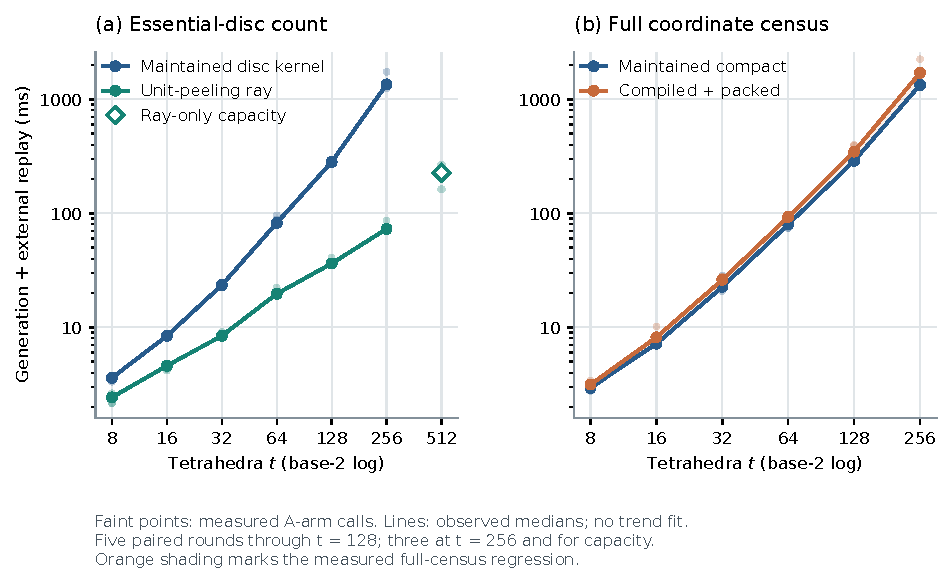
\includegraphics[width=\linewidth]{benchmarks.pdf}
\caption{Recorded generation plus independent external verification times.
The ray-disc specialization improves strongly on this family; the general
packed full-coordinate census does not.  Points are measured medians, with
no fitted asymptotic curve.  The new-ray-only 512-tetrahedron point is a
capacity measurement.}
\label{fig:benchmarks}
\end{figure}

\begin{figure}[tbp]
\centering
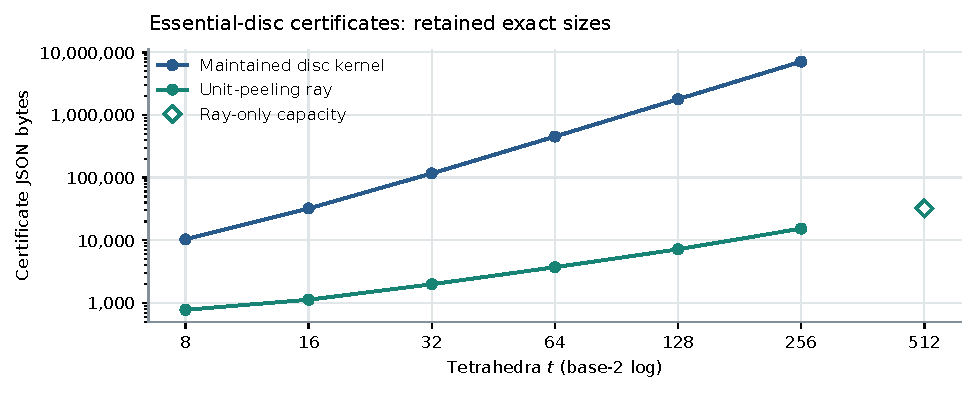
\includegraphics[width=0.88\linewidth]{proof_sizes.pdf}
\caption{Compact JSON disc-certificate sizes on the same family, excluding
source input.  The independently replayable unit-row transcript avoids the
large retained orbit trace.  The 512-tetrahedron diamond has no old-query
comparison; connecting lines only link measured values.}
\label{fig:proofsizes}
\end{figure}

\subsection{Negative and inconclusive performance findings}

\Cref{tab:coordinatetimes} is an essential qualification.  On the same
Fibonacci family the general packed census is slower at every measured size.
At $t=256$ the old census takes median $1335.527$ ms and the packed census
$1707.417$ ms, with old/new paired ratio $0.782$.  The new projection reduces
dimension from 256 to one, but the baseline already invokes its single-orbit
shortcut for weighted transport.  The common orbit discovery remains, and
general rank compilation adds cost.  A mathematically optimal slot budget
has not become a faster end-to-end query here.

The ray API also regresses on the three overhead controls in
\cref{tab:controls}: interior links, an interior sphere/disc/M\"obius mixture,
and a capped meridian with links.  The old primitive-core routine disposes of
these small cases cheaply.  The new conservative block construction, rank
gate, repeated geometry scans, and internal replay cost more than they save.
This is why the additions are explicit APIs, with no automatic replacement
of the default policy.

The isolated transport comparison holds the selected basis and unweighted
orbit trace fixed.  Vector/packed paired ratios are $0.953$, $1.004$, and
$1.042$ for the three controls.  The last has a broad paired range
$0.632$--$1.701$.  These observations validate the shared-run comparison but
do not establish a robust scalar-packing wall-clock advantage.  The capped
full census gives a small $1.087$ paired improvement, likewise too close to
the A/A variation to motivate a broad default change.

The practical conclusion is specific: the peeled rank-one disc gate is a
demonstrated improvement on the dense tested family.  The general observer
provides exact minimal dimension, optimal allocated bits, reusable rank
evidence, and a foundation for later work; current measurements do not justify
advertising it as a universal acceleration.

\subsection{Source-bound diagram stages}

\Cref{tab:diagramtimes} reports positive braid stabilizations of a circle:
the closure of $\sigma_1\sigma_2\cdots\sigma_n$ on $n+1$ strands.  The
maintained cocycle routine supplies a vector before timing.  The measured
stage constructs the canonical exterior, generates the new positive proof,
and independently checks its source binding.  All sizes through 32 crossings
and 640 exterior tetrahedra complete.  There is an A/A control but no old/new
recognizer comparison.  These inputs verify the source connection of the
new certificate path; they are not evidence that the complete recognizer is
faster on hard unknot diagrams.

\section{What remains between these results and quasi-polynomial recognition}
\label{sec:global}

The new local bounds are useful because they reduce the information transported
and sometimes avoid transport entirely.  They do not show how many source
supports recognition must try.  Even if every tested candidate is cheap,
exponentially many candidates would remain an exponential recognizer.

The following elementary accounting proposition states the required global
interface precisely.  It is a conditional composition statement, not a
verified property of the present recognizer.

\begin{proposition}[Conditional hierarchy accounting]
\label{prop:accounting}
Suppose a complete recognition procedure on an $n$-crossing input visits at
most $L(n)(g(n)+1)^{L(n)}$ hierarchy stages, where $L(n)\ge1$ and $g(n)\ge0$.
Charge all preprocessing, terminal work, failed attempts, and proof assembly
to these stages.  Suppose the total charged work at each
visited stage, including candidate selection, compressed updates, intermediate
representation, and independent checking, is at most $P(n)$.  Then its total
time is at most
\[
 L(n)(g(n)+1)^{L(n)}P(n).
\]
In particular, if $L(n)=O((\log n)^2)$, $g(n)=n^{O(1)}$, and
$P(n)=2^{O((\log n)^3)}$, the complete procedure takes
$2^{O((\log n)^3)}$ time.  The same conclusion holds with polynomial $P$.
\end{proposition}

\begin{proof}
Multiply the number of visits by the cost of a visit.  Its logarithm is at
most $\log L+L\log(g+1)+\log P$, which has the claimed order under the stated
hypotheses.  Work hidden in candidate selection or in an expanding intermediate
object must be included in $P$ for the implication to apply.
\end{proof}

The shape of the visit bound occurs in Lackenby's hierarchy analysis
\cite[Proposition~9.1]{Lackenby26}; verifying the stronger parameter hypotheses
for an implemented compressed recognizer is a separate research task.  Four
specific distinctions prevent an incorrect use of \cref{prop:accounting} here.

\begin{enumerate}
\item \textbf{A supplied vector versus a useful vector.}  Support nullity and
peeling are measured after the support has been supplied.  They do not identify
a meridian support among all admissible choices.
\item \textbf{A type inventory versus marked continuations.}  The bound
$H\le2d-a$ counts unmarked coordinate types.  A hierarchy can distinguish
boundary attachments, parallelity regions, and provenance not present in that
inventory.
\item \textbf{Small output versus cheap construction.}  A short rank witness
can still require expensive discovery on an arbitrary support; a compressed
cut can have short invariants but expensive attaching maps.
\item \textbf{A local budget versus a global budget.}  Restarting a successful
local procedure at every branch does not control the sum of its work.  A
monotone potential or a complete stage-count theorem is required.
\end{enumerate}

The diagram-exterior correspondence is already checked for the canonical
input construction.  The remaining source problem is maintaining comparable
provenance through the retriangulations and compressed cuts of a future
hierarchy.  Treating the input correspondence itself as wholly missing would
misdescribe the current repository.

\section{Further research questions and proposed theorem targets}
\label{sec:agenda}

The following programme separates near-term algorithmic work from the global
theorems that would change the asymptotic recognition result.  Each item names
an observable object or a falsifiable target.  Successful experiments may
motivate a theorem but do not replace one.

\subsection{Priority A: extend the provable local savings}

\paragraph{1. Multi-seed unit elimination with a controlled residual.}
When a one-seed closure stalls, introduce a new seed and express later exposed
coordinates as integral forms in the seeds.  The unsolved original rows then
give a residual system.  Can a seed-selection rule bound the number and width
of these forms by a structural parameter that stays small under relevant
layering and cutting operations?  A plausible target is a certified reduction
to $k$ residual variables in polynomial time with controlled coefficient bits.
One must not equate the number of greedy seeds with $d$: sparse exposure
closure is weaker than linear span closure.

\paragraph{2. Characterize and minimize single-seed stopping sets.}
View the supported matching rows as a bounded-arity incidence hypergraph.
Which connected normal supports admit a complete unit-peeling order?  Can
obstructions be characterized by a small core, and can that core be computed
without large integer elimination?  Seek families with $d=1$ but growing
unavoidable core size to delimit the shortcut's applicability.  Reordering
rows alone cannot solve every stopping-set obstruction.

\paragraph{3. Optimize a measured cost, beyond the slot sum.}
The present matroid theorem optimizes $L$, but exact decoder density and
coefficient height also cost time.  Can one choose an observer with a rigorous
bicriteria bound on slot budget and decoder sparsity?  A target could compare
to the best basis under $L+\lambda\nnz(N)$, or prove an approximation guarantee
under a sparse normal-matching structure.  The simple greedy proof does not
apply automatically to this nonadditive objective.

\paragraph{4. Make general rank compilation reusable under support edits.}
Hierarchies and candidate families often differ by a few zero coordinates.
Can a certified rank/decoder update handle a deletion or insertion of $k$
columns at cost polynomial in $k$ and the affected algebraic blocks, rather
than recompiling globally?  The verifier should check a small update against
the old certified matrix while preserving exact source support binding.

\paragraph{5. Prove a practical adaptive observer policy.}
Develop a preflight estimate comparing the old sparse $q+a$ decoder, the new
$d$ observer, and the ray gate.  A useful target is an overhead guarantee:
the dispatcher takes at most a small certified budget before reverting to the
baseline, and total time is bounded by that budget plus the selected complete
query.  The negative benchmark cases in this package provide a test set for
such a policy.  Prediction accuracy alone is not an asymptotic guarantee.

\subsection{Priority B: retain geometry and markings under compression}

\paragraph{6. A marked refinement of $H\le2d-a$.}
Specify exactly which markings a hierarchy needs on a component: boundary
arcs, attachment intervals, orientation data, and maps to the original
exterior.  Does a finite invariant of controlled bit length determine the
allowed next cuts?  Seek a bound on distinct marked states in terms of $d$
and marking complexity.  A counterexample with fixed $d$ and unbounded
necessary markings would be equally valuable.  Coordinate equality alone
is insufficient for this purpose.

\paragraph{7. Source-bound compressed cutting and gluing certificates.}
Realize existing compressed-cut mathematics as an executable source-bound
operation with an independent checker.  Lackenby's Theorem~14.4 already gives
polynomial cutting and parallelity-bundle attachment data for orientable
normal surfaces in uniform-type handle structures, in handle count and
logarithmic extended weight \cite{Lackenby26}.  The new target is a checked
representation in this architecture that carries the required source maps
through those operations.  The canonical input exterior checker is an
existing base case; later cuts require their own maps and verified hypotheses.

\paragraph{8. Stable local handle types and support complexity.}
Identify the precise class of handle structures produced by an implemented
hierarchy and prove that its operations preserve a uniform local incidence
bound.  Then determine how supported nullity, peeling cores, and marking size
change under those operations.  A theorem about arbitrary triangulations
cannot silently supply a bound for an expanding hierarchy representation.

\paragraph{9. Product-region removal with a charging argument.}
Can raw-support blocks, ray certificates, and two-sided profile types identify
parallelity/product regions that can be removed while charging every removal
to a decreasing potential?  The target is a global bound on cumulative
representation size and total local work, not just termination of each
individual removal.

\subsection{Priority C: close the global selection and hierarchy bounds}

\paragraph{10. Find a useful support without exhaustive support enumeration.}
Determine whether a meridian or hierarchy surface can always be found within
a quasi-polynomially bounded family of supports, after allowed checked
geometric preprocessing.  Possible parameters include a bounded exposure
core, support nullity, and normal boundary data.  The dense Fibonacci family
shows that few occupied quadrilateral positions are not necessary for easy
certification.  A low-nullity promise alone is not a discovery algorithm.

\paragraph{11. Quantify the limits of coherent cocycle candidates.}
The maintained minimum-span and Euler-optimal coherent cocycle family is not
a complete meridian family on arbitrary solid-torus triangulations, as proved
in \code{synthesis/coherent_obstruction.tex}.  That obstruction does not
establish failure on canonical diagram exteriors.  Formulate a controlled
enlargement that repairs identified obstructions and prove its candidate count
and bit-height bounds.  Re-running
the same optimizer with a new tie-breaker does not address a structural
incompleteness theorem.

\paragraph{12. Prove a polylogarithmic hierarchy potential.}
Seek a nonnegative potential on the complete marked state whose decrease
bounds the relevant hierarchy length by $O((\log n)^2)$, or by another
polylogarithmic function sufficient for \cref{prop:accounting}.  It must charge
all reset and branching operations.  A linear bound in a complexity parameter
that may itself grow polynomially in $n$ does not yield this conclusion.

\paragraph{13. A complete bit-complexity ledger.}
For every stage, bound the number of candidates, dimensions, coordinate
heights, decoder/certificate sizes, boundary maps, and repeated local calls.
Then compose the bounds without reinitializing the accounting at each branch.
The deliverable's source hashes and separated generation/replay timings are
small-scale infrastructure for this ledger; the missing proof is global.
For negative verdicts, seek shared certificates that exclude whole families
of failed support branches after unit substitutions.  A linear dual witness
can settle an individual convex cone, but a disjunction of quadrilateral
sectors requires evidence covering every alternative.  A certificate DAG
with shared substitution prefixes is a concrete target; a single failed
candidate is not a complete rejection argument.

\subsection{Priority D: falsification and validation}

\paragraph{14. Adversarial geometric families for overhead and core growth.}
Build genuine torus-boundary triangulations with large $d$, many supported
links, persistent exposure cores, and one-sided components.  Compare exact
costs before choosing a default policy.  Abstract sparse matrices test algebra
but cannot substitute for realizable normal-matching geometries when the
claim is geometric.

\paragraph{15. Formalize the smallest trusted lemmas first.}
The triangular unit-pivot lattice theorem and integer decoder identities are
compact candidates for a proof assistant or a very small extracted checker.
Next formalize raw-incidence block separation and the primitive ray disc
criterion.  Keep a traceability map from each formal statement to the concrete
certificate fields and finite manifold hypotheses.  This would strengthen
the independent Python checks without claiming that the present package is
already formally verified.

The immediate implementation order suggested by the evidence is an adaptive
local policy, multi-seed residual compilation, and a source-bound compressed
cut interface.  The highest-value mathematical target remains a selection
or hierarchy theorem controlling the complete marked state; local arithmetic
savings alone cannot supply it.

\appendix
\section{Reproduction and integration guide}
\label{sec:reproduce}

The archive is organized so that the mathematical report can be read
independently and the code can be reviewed as an additive change.  The
\code{repo_overlay/} tree contains new repository-relative files; the
\code{integration.patch} file describes the same additions.  A compact
\code{reference_snapshot/fast/} contains the pinned maintained Python source,
fixtures, and tests needed by these experiments, excluding historical result
archives, compiled caches, and unrelated large artifacts.  It is a source
subset, not a complete Git checkout.

The root reproduction script assembles a fresh run directory from the
reference snapshot and overlay, verifies its source provenance, and runs the
focused test suite or experiments.  It does not modify an existing checkout.
For a real integration, first check and apply the patch at the pinned commit,
review the nine added modules and five new test files, and run the included
commands.  The patch changes no existing production file.  Updating the
repository's synthesis index or incoming-work inventory is intentionally left
to the integration step requested by the user.

Python's standard library suffices for the new production code, focused tests
without optional geometric oracles, the algebra audit, and the benchmarks.
Regina~7.4 was used for the recorded geometric oracle run; install it separately
to repeat that oracle.  It is not bundled.  Matplotlib is only needed to
regenerate the plots.  A normal TeX installation with the listed packages
builds the article using two \code{pdflatex} passes; there is no external
bibliography download or shell-escape requirement.

\begin{lstlisting}[language=bash]
# From the unpacked archive root:
python3 reproduce.py --task tests
python3 reproduce.py --task audit --regina
python3 reproduce.py --task benchmark

# Or from an integrated fast/ directory:
python3 support_research/run_tests.py \
  --output support_research/results/local_regression.json
python3 support_research/audit.py --regina \
  --output support_research/results/local_audit.json
python3 support_research/benchmark.py --diagrams 1,4,8,16,32 \
  --output support_research/results/local_benchmark.json
\end{lstlisting}

The optional \code{--regina-path} argument points the audit and focused runner
at a separately installed Regina module; the runner propagates it to the
maintained subprocess integration tests.  Timings vary with hardware and
load.  Compare exact result hashes, successful replays, recorded scope, and
within-run paired ratios before comparing absolute milliseconds.

\section{Certificate schemas and executable contracts}
\label{sec:schemas}

The following descriptions are field-level guides; the independently written
checkers are the executable schema definitions.  Integers may use the exact
hexadecimal transport supported by the maintained codec.

\subsection{Supported matching kernel}
\begin{lstlisting}
schema: "normal-support-kernel-v1"
support, selected, pivots, pivot_rows
rank, nullity, denominator, numerators, modulus
\end{lstlisting}
\code{support} lists exactly the positive source indices.  The selected and
pivot lists partition it, with sizes $d$ and $r$.  The row list identifies the
claimed nonsingular original-row minor.  The numerator matrix is indexed by
support rows and selected-coordinate columns.  The checker verifies strict
indices, the identity block, all kernel equations, and modular unit-pivot
rank.  Optimality is a producer theorem; a valid nonoptimal decoder is still
valid evidence of the supplied profile calculation.

\subsection{Unit-exposed ray}
\begin{lstlisting}
schema: "normal-support-ray-peeling-v1"
support, seed, steps, nullity: 1
# Each step: [original_matching_row, newly_exposed_coordinate]
\end{lstlisting}
The checker reconstructs the source support, checks all source matching
equations, validates the seed, requires exactly $s-1$ steps, and checks the
one-unknown unit-pivot condition at every step.  Completion establishes the
integer ray theorem.  No list of primitive coefficients is needed in the
certificate; they are regenerated by the row recurrence when topology is
queried.

\subsection{Packed full-coordinate profile}
\begin{lstlisting}
schema: "normal-packed-components-v1"
input_sha256, encoding, support_kernel
boundary_homology_basis, weighted_orbits, summary
\end{lstlisting}
The encoding is either \code{packed} or \code{vector}, using the same selected
coordinates.  The source fingerprint binds the complete triangulation and
coordinates.  The orbit subcertificate uses the maintained weighted replay
format, whose unweighted trace key is \code{orbit_proof}.  Every decoded
component is integral, within source bounds, and classified from its recovered
complete vector.  The checker validates the total vector sum and all reported
multiplicities and disc counts.

\subsection{Geometric block disc count}
\begin{lstlisting}
schema: "normal-ray-block-disks-v1"
input_sha256, boundary_homology_basis, blocks
compressing_disk_components
\end{lstlisting}
The block list must equal the independently reconstructed raw-occurrence
partition.  A ray entry contains its support certificate, primitive divisor,
Euler characteristic, two boundary parity values, and disc count.  A fallback
entry contains the maintained complete disc-count certificate.  Counts are
checked block by block and summed.  No total number of connected components
is inferred from the primitive divisor.

\subsection{Positive knot-diagram evidence}
\begin{lstlisting}
schema: "diagram-ray-disks-v1"
input_pd, triangulation, coordinates, disc_certificate
\end{lstlisting}
The source checker requires the same normalized PD code, independently
verifies its canonical exterior, replays the disc certificate, and accepts
only a strictly positive count.  The producer returns \code{INCONCLUSIVE}
when the supplied vector has no essential disc.  Invalid geometry, invalid
coordinates, and corrupted proofs never become a negative knot verdict.

\section{A compact API example}

This example exercises an exponentially growing family while retaining a
short input vector and a short rank certificate.  It calls both the producer
and its independent checker.

\begin{lstlisting}[language=Python]
from normal_orbit_research.fixtures import layered_torus
from fastunknot.normal_ray_blocks import normal_ray_block_disk_count
from fastunknot.normal_ray_blocks_verify import (
    verify_normal_ray_block_disk_certificate,
)

triangulation, primitive = layered_torus(128)
multiplicity = (1 << 5000) + 1
source = [[multiplicity * x for x in row] for row in primitive]
answer = normal_ray_block_disk_count(
    triangulation, source, max_cycles=0, record_certificate=True,
)
assert answer["status"] == "COMPLETE"
assert answer["compressing_disk_components"] == multiplicity
assert answer["stats"]["orbit_cycles"] == 0
assert verify_normal_ray_block_disk_certificate(
    triangulation, source, answer["certificate"],
)
\end{lstlisting}

This invocation proves a fact about the supplied surface in the supplied
solid torus.  To assert a fact about a knot diagram, use the source-bound
wrapper with coordinates in that diagram's canonical exterior.  Supplying
coordinates from an unrelated triangulation is not a valid shortcut.

\clearpage
\section{Proof and evidence traceability}

\begin{longtable}{@{}>{\raggedright\arraybackslash}p{0.30\linewidth}>{\raggedright\arraybackslash}p{0.35\linewidth}>{\raggedright\arraybackslash}p{0.28\linewidth}@{}}
\toprule
Mathematical claim & Checked object & Main evidence \\
\midrule
\endhead
Minimum coordinate cost & Greedy pivot selection and exact decoder &
Exchange proof; exhaustive rational basis audits.\\[5pt]
Complete source reconstruction & $AN=0$, identity rows, nonsingular minor &
Independent modular replay and divisibility checks.\\[5pt]
Scalar transport equality & Common basis, original contribution fibres &
\Cref{thm:packing}; equal run statistics in every corpus case.\\[5pt]
Profile bound & Distinct disjoint types and horizontal doubles &
\Cref{thm:profile}; sharp one-sided and link fixtures.\\[5pt]
Geometric splitting & Original positive face-arc occurrences &
Independent adjacency reconstruction.\\[5pt]
Primitive connected ray & Rank-one support and integer primitivity &
Classical principle with explicit proof; one-sided tests.\\[5pt]
Integral unit ray & Triangular original-row transcript &
Independent unit-pivot replay; disabled generic paths.\\[5pt]
All Fibonacci sizes & Literal gluing recurrence and cell counts &
\Cref{thm:fibonacci}; finite implementation tests.\\[5pt]
Diagram-positive verdict & Canonical exterior plus positive disc proof &
Source mutation tests and canonical exterior checker.\\[5pt]
Global quasi-polynomial goal & Full marked search and transition bounds &
Conditional accounting only; open research agenda.\\
\bottomrule
\end{longtable}

The mathematical and software reviews corrected several overly broad draft
formulations: a symbolic cancellation pattern is not itself a geometric
counterexample; the double of a proper one-sided surface uses a horizontal
frontier; small support does not remove the implementation's full-array scan;
and coherent-cocycle obstructions on arbitrary solid-torus triangulations do
not imply an obstruction on canonical diagram exteriors.  These distinctions
are retained in the final statements and matter for future integration.


\clearpage
\begin{thebibliography}{99}
\raggedright
\bibitem{HLP99} J. Hass, J. C. Lagarias, and N. Pippenger.
 The computational complexity of knot and link problems.
 \emph{Journal of the ACM} 46 (1999), 185--211.
 \url{https://arxiv.org/abs/math/9807016}.
\bibitem{AHT06} I. Agol, J. Hass, and W. P. Thurston.
 The computational complexity of knot genus and spanning area.
 \emph{Transactions of the American Mathematical Society} 358 (2006), 3821--3850.
 \url{https://arxiv.org/abs/math/0205057}.
\bibitem{Edmonds71} J. Edmonds. Matroids and the greedy algorithm.
 \emph{Mathematical Programming} 1 (1971), 127--136.
 \url{https://doi.org/10.1007/BF01584082}.
\bibitem{Lackenby21Slides} M. Lackenby.
 \emph{Unknot recognition in quasi-polynomial time}. Oxford handout, March 2021.
 \url{https://people.maths.ox.ac.uk/lackenby/quasipolynomial-talk-oxford-compressed.pdf}.
\bibitem{Lackenby26} M. Lackenby.
 \emph{Incompressible surfaces, hierarchies and unknot recognition}.
 arXiv:2607.23350v1, 25 July 2026.
 \url{https://arxiv.org/abs/2607.23350v1}.
\bibitem{ProveIt} V. Reshetnikov, ProveIt repository and incoming research.
 Snapshot \code{3a90fb34146c915328ab8eac6250cc2514f74ed0}, inspected 9 October 2026.
 \url{https://github.com/VladimirReshetnikov/ProveIt}.
 The delivered provenance manifest identifies exact source blobs and archives.
\end{thebibliography}
\end{document}
